\documentclass[tikz,border=8pt]{standalone}
% Shared look for every TikZ diagram. Load with \input{../../tools/tikz-style.tex}
\usepackage[T1]{fontenc}
\usepackage{lmodern}
\renewcommand{\sfdefault}{lmr}  % diagrams use the same serif as the text
\usetikzlibrary{arrows.meta, positioning, shapes.geometric, calc, fit, backgrounds}
\definecolor{cblue}{HTML}{4C78A8}
\definecolor{corange}{HTML}{F58518}
\definecolor{cgreen}{HTML}{54A24B}
\definecolor{cred}{HTML}{E45756}
\definecolor{cpurple}{HTML}{B279A2}
\definecolor{cgrey}{HTML}{6B6B6B}
\tikzset{
  every picture/.style={font=\sffamily, line width=1.2pt},
  box/.style={draw=#1, fill=#1!12, rounded corners=4pt, align=center, inner sep=7pt, minimum height=1.1cm},
  box/.default=cgrey,
  arrow/.style={-{Stealth[length=3mm]}, draw=cgrey, line width=1.4pt},
  title/.style={font=\sffamily\bfseries\Large},
  note/.style={font=\sffamily\small, text=cgrey, align=center},
}
\AtBeginDocument{\hyphenpenalty=10000 \exhyphenpenalty=10000}

\begin{document}
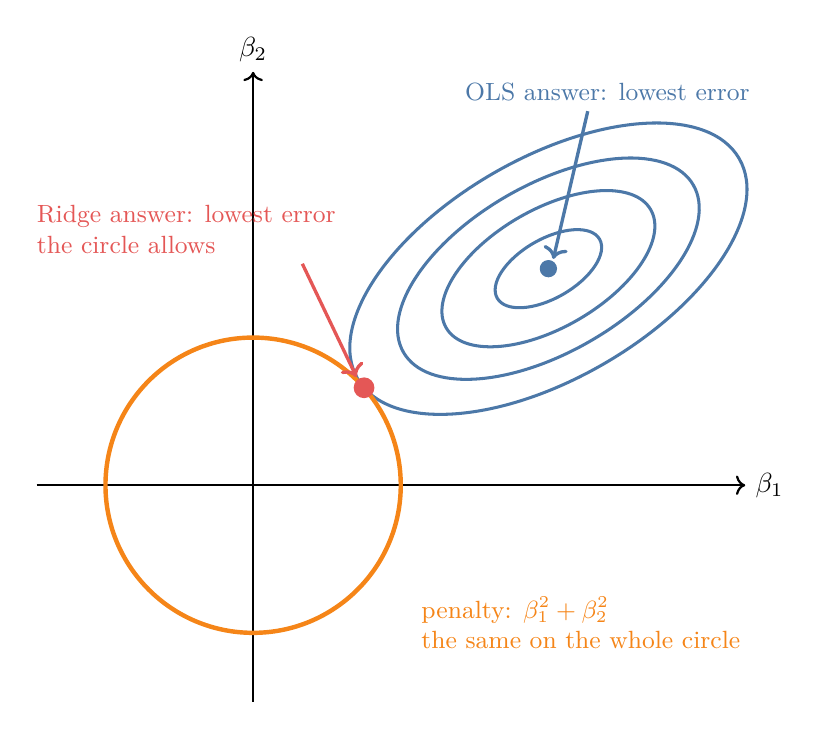
\begin{tikzpicture}[scale=1.25]
  \draw[->, thick] (-2.2,0) -- (5,0) node[right] {$\beta_1$};
  \draw[->, thick] (0,-2.2) -- (0,4.2) node[above] {$\beta_2$};
  % squared-error contours around the OLS answer
  \foreach \k/\o in {0.6/1, 1.2/1, 1.7/1, 2.238/1} {
    \draw[cblue, line width=1.1pt, opacity=\o, rotate around={30:(3,2.2)}] (3,2.2) ellipse ({\k} and {0.5*\k});
  }
  \fill[cblue] (3,2.2) circle (2.5pt);
  \node[note, text=cblue] at (3.6,4.0) {OLS answer: lowest error};
  \draw[cblue, ->] (3.4,3.8) -- (3.05,2.3);
  % penalty circle
  \draw[corange, line width=1.6pt] (0,0) circle (1.5);
  \node[note, text=corange, align=left, anchor=west] at (1.6,-1.4) {penalty: $\beta_1^2 + \beta_2^2$\\ the same on the whole circle};
  % touching point
  \fill[cred] (1.127,0.990) circle (3pt);
  \node[note, text=cred, align=left, anchor=east] at (0.95,2.6) {Ridge answer: lowest error\\ the circle allows};
  \draw[cred, ->] (0.5,2.25) -- (1.05,1.1);
\end{tikzpicture}
\end{document}
